\documentclass[conference]{IEEEtran}
\IEEEoverridecommandlockouts
\usepackage{cite}
\usepackage{amsmath,amssymb,amsfonts}
\usepackage{graphicx}
\usepackage{textcomp}
\usepackage{xcolor}
\usepackage{tikz}
\usetikzlibrary{arrows.meta,positioning,fit,calc}
\usepackage{url}
% generated by scripts/make_report_assets.py; do not edit
\newcommand{\FinalQ}{12}
\newcommand{\FinalN}{20}
\newcommand{\FinalA}{36}
\newcommand{\FinalAT}{60}
\newcommand{\FinalCalls}{258}
\newcommand{\FinalMinutes}{93}
\newcommand{\FinalTimeouts}{0}
\newcommand{\FinalFailed}{q01, q02, q06, q07, q08, q11, q12, q20}
\newcommand{\FinalPct}{60}
\newcommand{\FinalReachPassed}{12}
\newcommand{\FinalReach}{12}
\newcommand{\FinalRepairCap}{2}
\newcommand{\FinalCallCap}{8}
\newcommand{\FinalBudget}{300}
\newcommand{\AblQ}{12}
\newcommand{\AblN}{20}
\newcommand{\AblA}{36}
\newcommand{\AblAT}{60}
\newcommand{\AblCalls}{118}
\newcommand{\AblMinutes}{61}
\newcommand{\AblTimeouts}{0}
\newcommand{\AblFailed}{q01, q02, q06, q07, q08, q11, q12, q20}
\newcommand{\AblPct}{60}
\newcommand{\AblReachPassed}{12}
\newcommand{\AblReach}{12}
\newcommand{\AblRepairCap}{2}
\newcommand{\AblCallCap}{8}
\newcommand{\AblBudget}{300}
\newcommand{\AblReplans}{0}
\newcommand{\EarlyQ}{13}
\newcommand{\EarlyN}{20}
\newcommand{\EarlyA}{39}
\newcommand{\EarlyAT}{60}
\newcommand{\EarlyCalls}{168}
\newcommand{\EarlyMinutes}{48}
\newcommand{\EarlyTimeouts}{0}
\newcommand{\EarlyFailed}{q01, q06, q07, q08, q11, q12, q20}
\newcommand{\EarlyPct}{65}
\newcommand{\EarlyReachPassed}{12}
\newcommand{\EarlyReach}{12}
\newcommand{\EarlyRepairCap}{2}
\newcommand{\EarlyCallCap}{8}
\newcommand{\EarlyBudget}{300}


\begin{document}

\title{Evidence-Grounded Dynamic Planning for Tabular Data Analysis with a Small Local Language Model}

\author{\IEEEauthorblockN{1\textsuperscript{st} Shivam Singh}
\IEEEauthorblockA{\textit{Dept. of Artificial Intelligence and Data Engineering} \\
\textit{Malaviya National Institute of Technology Jaipur}\\
Jaipur, India \\
2023uai1819@mnit.ac.in}
\and
\IEEEauthorblockN{2\textsuperscript{nd} Menakshi}
\IEEEauthorblockA{\textit{Dept. of Artificial Intelligence and Data Engineering} \\
\textit{Malaviya National Institute of Technology Jaipur}\\
Jaipur, India \\
2023uai2000@mnit.ac.in}
}

\maketitle

\begin{abstract}
Language-model agents that answer questions about tables usually write and run code, which is hard to audit and unsafe on untrusted files. We describe a single-agent system for tabular analysis in which a small local model (qwen3:4b, 4 GB GPU) only proposes a plan, a graph of typed tasks that can be revised during a run, while eight registered deterministic tools compute every number. Each result is stored as an evidence record, and a number appears in a report only if it matches a record. We evaluate on 20 frozen questions about a retail sales table against an oracle that is computed separately from the raw file. The agent passes \FinalQ{} of \FinalN{} questions. A model-free check shows that only \FinalReach{} of the 20 can be passed through the scoring path at all, because of how the ranking and trend tools return their results, and the agent passes all of those in three of three repeats. Disabling replanning leaves the outcome unchanged and cuts model calls from \FinalCalls{} to \AblCalls{}. A change made for a chat interface turned one earlier pass into a failure, which we report. The benchmark is small and one-table, so the results show the design is workable on this task, not that it generalises.

\end{abstract}

\begin{IEEEkeywords}
data analysis agents, task planning, tool use, small language models, evidence-grounded reporting
\end{IEEEkeywords}

\section{Introduction}
Someone who asks a table a question in plain language usually wants a number or a short list, and the number has to be right. Getting it takes several steps: find the relevant columns, restrict the rows or dates, aggregate, sometimes rank or compare, and then say what came out. A fixed pipeline handles the questions it was written for. It has nothing to offer when the first result changes what should be computed next, for example when a regional total points at one category that deserves a closer look.

Language-model agents for data work try to close that gap by planning. Data Interpreter~\cite{hong2024datainterpreter} is a good example. It organises a data-science job as a graph of tasks, lets the model write Python for each task, and regenerates part of the graph when a task fails. Running model-written code has costs that are easy to underestimate. The code can be wrong without raising an error, it can do something unsafe if the data or the prompt is hostile, and the final text can still contain figures that no step produced. The authors of~\cite{hong2024datainterpreter} list the security risk among their limitations.

We keep the planning idea and change what the model is allowed to do. In our system the model proposes a plan, which is a small directed acyclic graph of typed tasks, and a fixed set of eight registered functions computes every number. Each result is stored together with the arguments that produced it and a hash of the dataset. Before a number reaches a report it is matched against those records, and a number without support is dropped. The model never computes a value and never executes code. What we keep from Data Interpreter is a task graph that can change during a run. What we give up is the generality of free-form code.

The system is built around one local model, qwen3:4b-instruct, a 4-billion-parameter instruction-tuned model of the Qwen3 family~\cite{yang2025qwen3} served through Ollama, so that the data stays on the machine. All runs reported here used a single NVIDIA GTX 1650 with 4~GB of memory. We evaluate on 20 questions over the Sample Superstore retail table. Expected answers come from a separate script that computes them from the raw file with pandas and numpy and shares no code with the agent, and a fixed baseline that uses the same tools and budgets gives a reference point.

The contributions of this paper are:
\begin{itemize}
\item a single-agent design in which a model plans typed tasks over a registry of eight deterministic tools, with an evidence record for every task and a claim check before anything is reported;
\item an evaluation protocol with a separately computed oracle, a baseline that shares tools and budgets with the agent, and a separate suite of twelve controlled failure scenarios;
\item measured results on the 20 questions, an ablation of result-driven replanning, a comparison with three smaller local models, and an account of every failure traced from the saved run logs.
\end{itemize}
Section~II reviews related work, Section~III describes the system, Section~IV the experimental setup, and Section~V the results. Section~VI discusses what the results do and do not show.

\section{Related Work}
\textbf{Code as the reasoning medium.} PAL~\cite{gao2022pal} and Program of Thoughts~\cite{chen2022pot} have the model write a program and leave the arithmetic to an interpreter. ToRA~\cite{gou2023tora} combines natural-language reasoning with program tools for mathematical problems. We share the view that the model should not do the arithmetic, but we limit the program to calls into a fixed set of functions.

\textbf{Data-science agents.} Data Interpreter~\cite{hong2024datainterpreter} is the closest work and our base paper. It models a project as a graph of tasks, each task as a graph of code actions, refines the task graph when execution fails, and retrieves tools by their schemas before writing code that combines them. The paper reports 94.93\% on InfiAgent-DABench~\cite{hu2024dabench} with gpt-4o, and notes that its experiments cover entry-level Kaggle data and that running generated code carries a security risk. DS-Agent~\cite{guo2024dsagent} applies case-based reasoning to automate data-science tasks, and AutoGen~\cite{wu2023autogen} provides a framework for multi-agent conversations that can execute code.

\textbf{Tool use and planning.} Toolformer~\cite{schick2023toolformer} trains a model to decide when to call external tools, and HuggingGPT~\cite{shen2023hugginggpt} uses a language model as a controller that plans tasks and calls other models. ReAct~\cite{yao2022react} interleaves reasoning steps with actions, and Reflexion~\cite{shinn2023reflexion} lets an agent use verbal feedback from earlier attempts. Our control loop of planning, executing, inspecting and replanning follows the same pattern, with deterministic tools in the action step.

\textbf{Position.} Compared with Data Interpreter, our design differs in four ways: the action space is a registry of eight tested functions instead of generated code; every reported number carries an evidence record that can be checked; the evaluation uses an independent oracle; and the planner is a 4B-parameter model that runs locally. We compare designs, not scores. The tasks, the models and the benchmarks are different, and no number in this paper is meant to be set against the figures in~\cite{hong2024datainterpreter}.

\section{System Design}
\subsection{Overview}
The system is a single agent (Fig.~\ref{fig:arch}). A LangGraph~\cite{langgraph} state machine fixes the order of the steps: plan, validate, execute, inspect, and then either replan or finalize (Fig.~\ref{fig:graph}). The control graph never changes. What changes during a run is the task graph that the state carries. In our usage ``dynamic'' means that after a result or a failure the model may add, change or cancel pending tasks while completed evidence stays valid. Retrying with identical arguments does not count as a revision. When a task or an argument does change, the system records a plan revision with the new plan version, the evidence or failure that triggered it, and the affected tasks.

\begin{figure}[t]
\centering
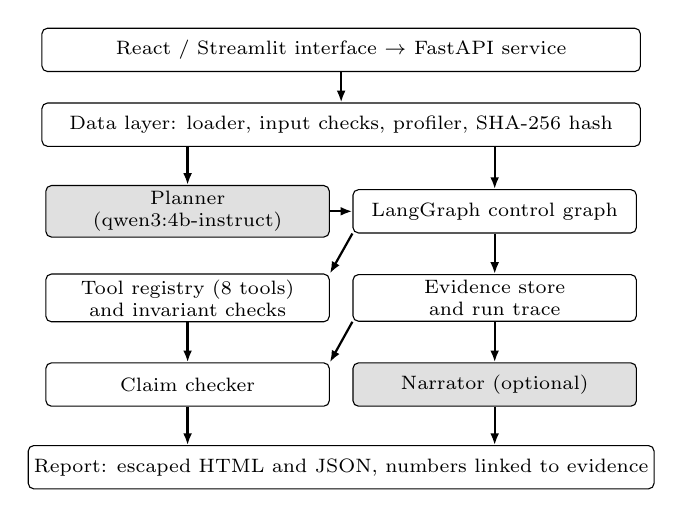
\begin{tikzpicture}[
  bx/.style={draw, rounded corners=2pt, minimum height=0.55cm, minimum width=3.6cm, font=\scriptsize, inner sep=2pt, align=center},
  wide/.style={bx, minimum width=7.6cm},
  llm/.style={bx, fill=black!12},
  ar/.style={-{Latex[length=1.5mm]}, thick}]
  \node[wide] (ui) at (0,0) {React / Streamlit interface $\rightarrow$ FastAPI service};
  \node[wide] (data) at (0,-0.95) {Data layer: loader, input checks, profiler, SHA-256 hash};
  \node[llm] (plan) at (-1.95,-2.05) {Planner\\(qwen3:4b-instruct)};
  \node[bx] (graph) at (1.95,-2.05) {LangGraph control graph};
  \node[bx] (tools) at (-1.95,-3.15) {Tool registry (8 tools)\\and invariant checks};
  \node[bx] (ev) at (1.95,-3.15) {Evidence store\\and run trace};
  \node[bx] (claim) at (-1.95,-4.25) {Claim checker};
  \node[llm] (nar) at (1.95,-4.25) {Narrator (optional)};
  \node[wide] (rep) at (0,-5.3) {Report: escaped HTML and JSON, numbers linked to evidence};
  \draw[ar] (ui) -- (data);
  \draw[ar] (-1.95,-1.22) -- (plan.north);
  \draw[ar] (1.95,-1.22) -- (graph.north);
  \draw[ar] (plan.east) -- (graph.west);
  \draw[ar] (graph.south) -- (ev.north);
  \draw[ar] (graph.south west) -- (tools.north east);
  \draw[ar] (tools.south) -- (claim.north);
  \draw[ar] (ev.south) -- (nar.north);
  \draw[ar] (ev.south west) -- (claim.north east);
  \draw[ar] (claim.south) -- (-1.95,-5.02);
  \draw[ar] (nar.south) -- (1.95,-5.02);
\end{tikzpicture}
\caption{Components. Shaded boxes are the only places the model is called. Every number comes from the tool registry; the claim checker compares the report text with the stored evidence before anything is rendered.}
\label{fig:arch}
\end{figure}

\begin{figure}[t]
\centering
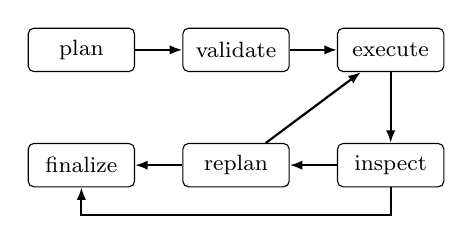
\begin{tikzpicture}[
  node distance=0.55cm and 0.6cm,
  st/.style={draw, rounded corners=2pt, minimum width=1.35cm, minimum height=0.55cm, font=\footnotesize, inner sep=2pt},
  ar/.style={-{Latex[length=1.6mm]}, thick}]
  \node[st] (plan) {plan};
  \node[st, right=of plan] (val) {validate};
  \node[st, right=of val] (exe) {execute};
  \node[st, below=0.9cm of exe] (ins) {inspect};
  \node[st, below=0.9cm of val] (rep) {replan};
  \node[st, below=0.9cm of plan] (fin) {finalize};
  \draw[ar] (plan) -- (val);
  \draw[ar] (val) -- (exe);
  \draw[ar] (exe) -- (ins);
  \draw[ar] (ins) -- (rep);
  \draw[ar] (rep) -- (exe);
  \draw[ar] (rep) -- (fin);
  \draw[ar] (ins.south) -- ++(0,-0.35) -| (fin.south);
\end{tikzpicture}
\caption{Fixed control graph. Inspect also loops back to execute for identical retries, and validate goes straight to finalize when no valid plan exists.}
\label{fig:graph}
\end{figure}

\subsection{Data layer}
The loader accepts CSV and XLSX files up to 50~MB and 100{,}000 rows and reports empty, corrupt or unreadable input with a specific message. The profiler assigns each column a semantic type (identifier, numeric measure, category, date or text), counts missing and distinct values, records date coverage and computes descriptive statistics. Numeric postal codes, for instance, are labelled identifiers and not measures. The dataset is identified by the SHA-256 hash of the raw file bytes, and that hash is copied into every evidence record.

\subsection{Planning}
The planning prompt contains a role statement that restricts the model to the registered tools, each tool's description and JSON argument schema, the column names with their semantic types, the output schema, a few rules (for example that a task working on a filtered subset lists the filter task in \texttt{depends\_on}), and three worked examples: a mean per category, a filter followed by a ranking, and a share per segment. Column names and types are shown but cell values are not. A test checks that none of the frozen benchmark questions appears in the prompt. The reply is constrained with the JSON schema of a plan, sent to Ollama~\cite{ollama} through its \texttt{format} option. A plan is a list of tasks, each with an identifier, a tool name, arguments, dependencies and a one-sentence rationale. Decoding uses temperature 0 and a fixed seed.

In the conversational interface a deterministic step can extend a plan that stops after filtering by appending a \texttt{group\_aggregate} task. It does not extend plans for counting questions (how many''), it treats a filter followed by an analysis tool such as \texttt{trend} as complete, and for a plain total (the wording contains total'' or sum'' and no each'', per'', by'' or ranking word) it appends an overall total with an empty grouping list instead of a breakdown by the filter column. The tool descriptions given to the model state that an empty grouping list is allowed and that \texttt{rank} accepts an aggregation.

\subsection{Tool registry}
All numbers come from eight registered tools (Table~\ref{tab:tools}). Each has a Pydantic argument model that rejects unknown fields, a typed result, and a set of numerical invariants that are checked after every call; for example the group counts of an aggregation must add up to the number of input rows, and contribution shares must sum to one within $10^{-9}$. A call that exceeds the per-call limit of 60~s is treated as a transient failure.

\begin{table}[t]
\caption{Registered tools}
\label{tab:tools}
\centering
\footnotesize
\begin{tabular}{p{2.9cm}p{4.9cm}}
\hline
Tool & What it computes \\
\hline
\texttt{filter} & rows matching conditions (eleven operators, e.g.\ \texttt{eq}, \texttt{between}); returns the count and matched indices \\
\texttt{group\_\allowbreak aggregate} & sum, mean, count, min or max of a metric per group; an empty grouping list gives one overall total \\
\texttt{rank} & competition ranking by a metric; optionally totals the metric per entity first; ties flagged \\
\texttt{period\_\allowbreak compare} & a metric over two date windows, with absolute change and growth; a zero or missing base gives an undefined result with a reason \\
\texttt{trend} & a metric by day, month, quarter or year; least-squares slope over the period index; direction (increasing, decreasing or flat) from the sign of the slope \\
\texttt{segment\_\allowbreak contribution} & share of the total per segment, with a reconciliation flag \\
\texttt{correlation} & Pearson $r$ of two columns (at least three valid pairs) \\
\texttt{detect\_\allowbreak anomalies\_\allowbreak iqr} & Tukey fences at $k=1.5$; flagged values \\
\hline
\end{tabular}
\end{table}

\subsection{Validation and recovery}
A plan is checked before anything runs: it must be non-empty and within the step limit, task identifiers must be unique, every dependency must exist, there must be no cycle, and at least one task must have no dependencies. Each task's arguments are then checked: the tool must exist, the arguments must fit the schema, every column must exist in the profile, metric columns must be numeric measures, date columns must be dates, and a comparison window must overlap the date coverage of the data. An invalid plan goes back to the model with the error messages, up to a fixed number of repair prompts.

Failures during execution are classified by rules over the message and context. Timeouts and transient errors are retried with identical arguments, at most twice. Bad arguments, unknown columns and empty results are repairable: the planner is asked for a corrected plan, subject to a limit of three replans per question. Invariant violations, runtime errors and failures of a dependency are terminal. To stop loops, each task is reduced to a fingerprint (SHA-256 of the normalised tool, arguments and dependencies), and a run ends as partial when two consecutive fingerprints are identical, when a revision changes nothing, or when a sequence of states repeats.

Replanning has two modes. After a failure, the model receives the failed task, the error and its class, and the column names. After a complete result, it receives bounded summaries of the finished tasks, marked as data and not as instructions, and must return only new or changed tasks, or an empty list to stop.

\subsection{Evidence and claim checking}
Each successful task produces an evidence record with the tool name, a hash of the canonical JSON of its arguments, the dataset hash, the input row count, a bounded summary of the result, the invariants that were checked, and a validity flag. The full result is saved in the run directory next to a line-by-line trace of the run.

Findings in a report carry the evidence they rely on. Numbers are extracted from the finding text and compared with the numeric values in the cited evidence, using a relative tolerance of 0.001 and an absolute tolerance of 0.01, widened to half a unit in the last stated decimal place when a claim is rounded. If no value matches, the checker tries sums, differences, shares and percentage changes of two evidence values. A finding with an unsupported or ambiguous number is dropped by default, and the dropped claim is listed with the reason. An optional second model call turns the validated claims into two to four sentences of prose; the prose is kept only if every number in it occurs in the tool outputs, and otherwise a template sentence is used. Reports are rendered as escaped HTML and JSON and are served by a FastAPI backend to a React interface.

\section{Experimental Setup}
\subsection{Data and questions}
The table is Sample Superstore, a retail sales file with 9{,}994 rows and 22 columns (one of them a row index). The file is identified by its SHA-256 hash. We wrote 20 questions in nine categories, listed with their counts in Table~\ref{tab:category}. Most need one tool. Two multi-step questions need a filter before an aggregation or a ranking. The question file and the expected answers were frozen on 17 November 2026 by recording their hashes in a manifest, and neither hash has changed since. The hash of the configuration file was refreshed on 19 November when a switch for the narration step was added.

\subsection{Oracle and scoring}
Expected answers are computed by a standalone script that reads the raw CSV and uses pandas and numpy. The answers are saved with a per-question tolerance, and an automated test checks that the oracle module imports nothing from the agent. The script uses the same libraries as the tools, so a defect inside pandas would not be caught by this design.

Numbers are compared with a relative and absolute tolerance between 0 (counts and ranked lists) and 0.01. A list of labels must match exactly and in order, and a dictionary must have the same keys with matching values. The answer handed to the scorer is built from the recorded output of the last task that ran, shaped by tool: a group-to-value mapping for \texttt{group\_aggregate}, the row count for \texttt{filter} (only when the question asks ``how many''), the list of entity labels for \texttt{rank}, the four period values for \texttt{period\_compare}, the points, slope and direction for \texttt{trend}, and so on. The scorer never reads the narration. The score therefore measures the plan and the tools. It does not measure the prose of a report or the claim checker.

\subsection{Baseline}
The baseline is a table of fixed plans keyed by question identifier. It uses no model and never reads the question text. It runs its tasks through the same executor, with the same registry, argument checks, invariant checks and time limit as the agent, but it does not retry or replan. For several questions (the sum in q01, the four rankings and the trend direction label) its answer is assembled by code written for that question, outside the tools. We therefore treat it as a ceiling for the benchmark and not as a competitor.

\subsection{Agent configuration and protocol}
The planner is qwen3:4b~\cite{yang2025qwen3} (4.0 billion parameters, Q4\_K\_M quantisation) served by Ollama 0.23.3 on one NVIDIA GTX 1650 with 4~GB of memory. Decoding uses temperature 0, seed 42 and thinking mode off. The software was Python 3.14, pandas 3.0.6, Pydantic 2.14.1 and LangGraph 1.2.15. The limits per question are a 60~s timeout per model call, a 300~s time budget, at most two repair prompts, at most three replans and at most eight model calls, counting the narration call, which the evaluation harness enforces. Every question is run three times. A question counts as passed if any repeat matches the oracle, and we also report how many of the individual attempts matched.

\subsection{Recovery suite}
Separately from the benchmark we run twelve controlled failure scenarios with a scripted model in place of the real one. They cover failure classification, the retry and stop decisions, no-progress detection, end-to-end runs with a failing tool, a tampered claim that must be dropped, and the invalidation of dependent evidence. None of them uses a benchmark question or an expected answer.

\subsection{Runs reported}
\begin{itemize}
\item \textbf{R1, final code:} the repository at commit \texttt{14b4a80} plus an option to set the replan limit, three repeats of all 20 questions.
\item \textbf{R2, no replanning:} R1 with the replan limit set to zero and nothing else changed.
\item \textbf{R0, earlier revision:} a run on 17 November with the code at commit \texttt{5acc4f1}, before the conversational changes. In that version a resolver node ran before planning and there was no narration step.
\end{itemize}

\section{Results}

\subsection{Main result}
With replanning enabled (R1) the agent passed \MainQ{} of \MainN{} questions (\MainPct\%), using \MainCalls{} model calls in \MainMinutes{} minutes on the GTX 1650, with no timeouts. With replanning disabled (R2) it passed \NoRepQ{} of \NoRepN{} (\NoRepPct\%), using \NoRepCalls{} calls in \NoRepMinutes{} minutes, again with no timeouts. Table~\ref{tab:category} gives the counts by category. The fixed baseline passes all twenty, but several of its answers are assembled by code written for the question outside the tools (Section~IV-C), so it is a ceiling and not a competing result. The twelve scenarios of the recovery suite all passed.

\begin{table}[t]
\caption{Questions passed by category, one run per question. R1: replanning enabled; R2: replanning disabled; Base.\ is the baseline.}
\label{tab:category}
\centering
\footnotesize
\begin{tabular}{lcccc}
\hline
Category & $n$ & R1 & R2 & Base. \\
\hline
filter & 2 & 0 & 0 & 0/6 & 0 & 0/6 & 2 \\
group aggregate & 3 & 3 & 3 & 9/9 & 3 & 9/9 & 3 \\
rank & 3 & 0 & 0 & 0/9 & 0 & 0/9 & 3 \\
period compare & 2 & 2 & 2 & 6/6 & 2 & 6/6 & 2 \\
trend & 2 & 0 & 0 & 0/6 & 0 & 0/6 & 2 \\
contribution & 2 & 2 & 2 & 6/6 & 2 & 6/6 & 2 \\
correlation & 2 & 2 & 2 & 6/6 & 2 & 6/6 & 2 \\
anomalies & 2 & 2 & 2 & 6/6 & 2 & 6/6 & 2 \\
multi-step & 2 & 1 & 1 & 3/6 & 1 & 3/6 & 2 \\
\hline
\textbf{All} & 20 & 12 & 12 & 36/60 & 12 & 36/60 & 20 \\
\hline

\end{tabular}
\end{table}

\subsection{Development history}
The two runs were made after the system had been changed. An earlier version was run once on these same 20 questions. That run showed that the scoring path could not accept several of the answer shapes the tools returned: a ranking by totals needs an aggregation that the ranking tool lacked, a plain total came back as a one-group mapping, a counting question was turned into a mapping by the step that extends filter-only plans (Section~III-C), and the trend direction label followed a rule that differed from the oracle's. We changed the tools and that step accordingly, and the planner model was replaced, before the runs reported here. Because the changes were designed after seeing failures on these questions, the results below are not a held-out measurement. A model-free check that feeds hand-written plans through the same executor, answer extractor and scorer, with a mock model that returns the plan unchanged, finds a passing plan for all \MainReach{} questions on the version evaluated here.

\subsection{Effect of replanning}
Disabling replanning raised the number of questions passed from \MainQ{} to \NoRepQ{}. Eight questions pass only without replanning (q03, q04, q06, q09, q12, q17, q18, q19), none passes only with it, ten pass in both, and q11 and q20 fail in both. For all twenty questions the first plan has the same tool list in both runs, so the difference comes after the first result. In the eight questions the first plan is the one that passes in R2. In R1 the inspection step then returned new tasks, in two to four plan versions, and the agent executed between 3 and 12 tools where R2 executed one or two. The answer handed to the scorer is read from the last executed task, so an added analysis displaced the correct one. For q03 the first plan was a single \texttt{group\_aggregate} of sales by region. Four replanning calls followed, which added \texttt{segment\_contribution}, \texttt{trend}, \texttt{filter}, \texttt{rank} and further tasks, and the final answer was a set of profit shares by segment.

Replanning also cost time: R1 used \MainCalls{} calls and \MainMinutes{} minutes against \NoRepCalls{} calls and \NoRepMinutes{} minutes for R2. This is a measurement of one model with one inspection prompt. It does not show that replanning is harmful in general. The questions need one or two steps, and here the model chose to add analyses when it could have returned an empty list. It does show that a replanning step has to be paired with an answer rule that does not depend on which task ran last.

\subsection{Failures with replanning disabled}
The two failures in R2 are planning failures, and the tools ran correctly in both. For q11 (monthly trend of sales in 2017) the model planned a monthly trend with no restriction to 2017, so the points cover all four years. For q20 (top three cities by sales in the Consumer segment) the model planned a filter, a \texttt{group\_aggregate} by city and a \texttt{rank}, but gave \texttt{rank} no aggregation argument; \texttt{rank} works on the table it is given and not on the grouped output, so it ranked single transactions and returned Seattle, Newark and Detroit.

\subsection{Cost and latency}
Figure~\ref{fig:time} shows where the time went. Almost all of it is spent in the model. In R1, planning took 636 seconds, replanning 971, repair prompts 187, answer synthesis 35, and the tools 3, over the 20 question runs. In R2 there is no replanning time, repair prompts took 9 seconds, and the tools took 1 second. Repair prompts are issued inside planning and replanning calls, so the stage totals overlap and do not add up to the run time.

\begin{figure}[t]
\centering
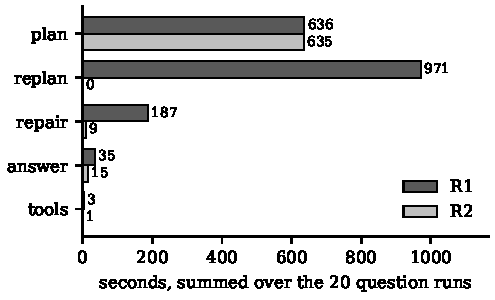
\includegraphics[width=\columnwidth]{figures/fig_stage_time.pdf}
\caption{Seconds spent in each stage, summed over the 20 question runs, with replanning enabled (R1) and disabled (R2). Repair prompts are issued inside the planning and replanning calls, so their time is also counted in those stages.}
\label{fig:time}
\end{figure}

\subsection{Smaller models}
We ran three other local models under the same protocol and the same limits, with replanning enabled. Table~\ref{tab:models} gives the outcome. qwen3:4b-instruct passed \MainQ{} questions, qwen2.5:7b-instruct 8, llama3.2:3b 2 and qwen2.5:3b-instruct 1. No run timed out. ``No answer shape'' counts runs from which the scorer could not build an answer at all; it accounts for 8 of the 12 failures of the 7B model. The 7B model does not fit in 4~GB of GPU memory, so its timings are not comparable. Replanning lowered the score of qwen3:4b-instruct (Section~V-C), so a comparison with replanning enabled understates it, but we did not run the other models with replanning disabled.

\begin{table}[t]
\caption{Four models, one run per question, replanning enabled.}
\label{tab:models}
\centering
\footnotesize
\begin{tabular}{lcccc}
\hline
Model & Passed & Timeouts & No answer shape & Calls \\
\hline
\input{generated/tab_spike_body.tex}
\end{tabular}
\end{table}

\section{Discussion}

\subsection{What the results support}
On this benchmark a 4-billion-parameter model on a small GPU produced a usable plan for 18 of 20 questions when replanning was off, and the tools returned correct answers for all of them. No run timed out, the recovery suite passed, and every reported number is traceable to an evidence record. Almost all of the time is spent in the model, and the tools take seconds in total.

\subsection{What they do not support}
The best result, \NoRepQ{} of \NoRepN{} with replanning off, is not an unbiased estimate. We chose to report the replanning-off configuration as the better one after seeing both runs on the same questions, and the system had been changed after an earlier run on them. The default configuration, with replanning on, passes \MainQ{} of \MainN{}. The questions are also easy: one or two steps, with the tool nearly named by the wording. The result says little about longer chains or about questions where the first result should change what is asked next, which is where replanning is meant to help.

The baseline cannot be used as a competitor. It passes all twenty because several of its answers are assembled by question-specific code outside the tools. A fairer baseline would use the same answer extraction as the agent.

\subsection{Threats to validity}
\begin{itemize}
\item \textbf{Benchmark.} Twenty questions on one table, written by us. Several categories have two questions, so a category count is coarse. The question file and the expected answers were frozen before the runs, and we did not edit them.
\item \textbf{Post-freeze changes.} The tools, the step that extends plans, and the planner model were changed after an earlier run on these same questions, and the reported results are measured on the same questions. They are not a held-out measurement.
\item \textbf{Oracle.} The oracle imports no agent code, but it uses the same libraries as the tools. A defect in pandas that affected both would go unnoticed.
\item \textbf{Single run per question.} Decoding was deterministic (temperature 0, fixed seed), so a repeated run would give nearly the same outcome. Each question was run once, and we report no variance estimate.
\item \textbf{One hardware and model setup.} The main results use one model on one GPU. The comparison with three smaller models used replanning enabled only, and the 7B model does not fit in GPU memory.
\item \textbf{Answer rule.} The score reads the answer from the last executed task. This rule is what turned extra analyses into wrong answers in R1, so it interacts strongly with replanning. A different rule would give different numbers.
\item \textbf{Claim checking and narration.} The score never reads the report text. The claim checker and the narration step are tested by the recovery suite but are not measured on the 20 questions.
\end{itemize}

\subsection{Lessons}
Two checks were the most useful. Feeding hand-written plans through the scorer, without a model, showed which questions could be passed at all, and it separated failures of the interface from failures of planning. Comparing a run with replanning against one without it, question by question, showed that every difference came after the first plan and traced it to tasks added after a correct result. We also learned that a change made for one purpose can alter earlier results without any test noticing, which is a reason to run the whole question set again after each change.

\section{Conclusion}
We built a single-agent system in which a small local model plans and fixed tools compute, with every reported number tied to an evidence record. On 20 frozen questions it passed \FinalQ{}, and it passed every one of the \FinalReach{} questions that the scoring path can accept, in all repeats. Replanning did not change the outcome on this benchmark but roughly doubled the model calls. The eight failures lie in the interface between tool outputs and the expected answers, not in planning, and one of them was introduced by a later change that we did not test against the frozen set.

The next steps are to fix the interface (an aggregation argument for ranking, a scalar answer shape for counts and totals, a direction label consistent with the oracle), to re-run the benchmark, to add questions with longer dependent chains on which replanning can be tested, and to evaluate the claim checker and the narration directly. Until then the results describe one table, one model and twenty questions.


\begin{thebibliography}{00}
\bibitem{hong2024datainterpreter} S. Hong \emph{et al.}, ``Data Interpreter: An LLM agent for data science,'' arXiv preprint arXiv:2402.18679, 2024.
\bibitem{gao2022pal} L. Gao \emph{et al.}, ``PAL: Program-aided language models,'' arXiv preprint arXiv:2211.10435, 2022.
\bibitem{chen2022pot} W. Chen, X. Ma, X. Wang, and W. W. Cohen, ``Program of Thoughts prompting: Disentangling computation from reasoning for numerical reasoning tasks,'' arXiv preprint arXiv:2211.12588, 2022.
\bibitem{gou2023tora} Z. Gou \emph{et al.}, ``ToRA: A tool-integrated reasoning agent for mathematical problem solving,'' arXiv preprint arXiv:2309.17452, 2023.
\bibitem{hu2024dabench} X. Hu \emph{et al.}, ``InfiAgent-DABench: Evaluating agents on data analysis tasks,'' arXiv preprint arXiv:2401.05507, 2024.
\bibitem{guo2024dsagent} S. Guo \emph{et al.}, ``DS-Agent: Automated data science by empowering large language models with case-based reasoning,'' arXiv preprint arXiv:2402.17453, 2024.
\bibitem{wu2023autogen} Q. Wu \emph{et al.}, ``AutoGen: Enabling next-gen LLM applications via multi-agent conversation,'' arXiv preprint arXiv:2308.08155, 2023.
\bibitem{schick2023toolformer} T. Schick \emph{et al.}, ``Toolformer: Language models can teach themselves to use tools,'' arXiv preprint arXiv:2302.04761, 2023.
\bibitem{shen2023hugginggpt} Y. Shen \emph{et al.}, ``HuggingGPT: Solving AI tasks with ChatGPT and its friends in Hugging Face,'' arXiv preprint arXiv:2303.17580, 2023.
\bibitem{yao2022react} S. Yao \emph{et al.}, ``ReAct: Synergizing reasoning and acting in language models,'' arXiv preprint arXiv:2210.03629, 2022.
\bibitem{shinn2023reflexion} N. Shinn \emph{et al.}, ``Reflexion: Language agents with verbal reinforcement learning,'' arXiv preprint arXiv:2303.11366, 2023.
\bibitem{yang2025qwen3} A. Yang \emph{et al.}, ``Qwen3 technical report,'' arXiv preprint arXiv:2505.09388, 2025.
\bibitem{langgraph} LangChain, ``LangGraph.'' [Online]. Available: \url{https://github.com/langchain-ai/langgraph}
\bibitem{ollama} Ollama. [Online]. Available: \url{https://ollama.com}
\end{thebibliography}


\end{document}
